\documentclass[a4paper,11pt]{article}

\usepackage{graphicx,fullpage}
\usepackage{listings}


%opening
\title{Dataflow Analysis for Irregular Programs.\\FADA Toolkit User's Guide}
\author{Marouane \textsc{Belaoucha} and Denis \textsc{Barthou} and Sid-Ahmed-Ali \textsc{Touati}\\
University of Versailles Saint-Quentin en Yvelines, France
}
\begin{document}
\lstset{language=C++,
	basicstyle=\scriptsize,
	keywordstyle=\bfseries,
	numbers=left,
	numberstyle=\tiny,
	frameround=fttt
	}

\maketitle

\begin{abstract}
Usual data dependence analysis works for a restricted set of programs, mainly the so called static control programs. However, usual C codes fragments for instance do not fit in this class of programs,  consequently current compilers do not have precise data dependence analysis for them. With the future massive introduction of multicore processors, desktop applications become the future candidate for code analysis and automatic parallelisation. In this context, FADA extends the array data dependence analysis to take into account irregular code structures such that while-loops, function calls, non affine array accesses, if-then-else, etc. Fuzzy Array Dependence Analysis (FADA) is more powerful but requires more compilation time. Other applications are also possible and are described in \cite{d2.3.2}.

We present a user documentation for the FADA toolkit. FADA toolkit is a partial C++ implementation of the FADA analysis \cite{barthou_thesis}. It is an instance wise dependence analysis for non static control programs, commonly called irregular codes. \verb|FADAlib| is its C++ API, allowing its usage a library for compilers and code analysers. \verb|FADAtool| is the command line tool of the FADA toolkit. This manual shows how to use\verb|FADAlib| and  \verb|FADAtool|.
\end{abstract}
\tableofcontents

\section{Introduction}

\subsection{What is FADA Toolkit ?}
 {\it FADA Toolkit} is a partial implementation of the FADA (Fuzzy Array Dataflow Analysis), which is an instance-wise dependence analysis for non static control programs, sometimes called {\it irregular} programs. The advantages of FADAlib are:

\begin{itemize}
    \item It extends the Feautrier's ADA analysis \cite{ada_feautrier}, so it has full support for static control programs.
    \item It provides support for many kinds of control flow irregularities, resulting in better precision for data flow analysis. Such irregularities may be on memory accesses (indirection, non-affine indexes) and on irregular control structures (while, if-then-else). In some cases, FADA can provide more precise analysis results, while the classical ADA approach simply fail to take onto account these control structures.
\end{itemize}

For detailed information about the FADA analysis, please refer to FADA Toolkit website \cite{fadalib_website}.

\subsection{Definitions}
Here, we summarise some recurrent terms used in the literature and this manual.
\begin{description}
 \item[Parameters or symbolic constants] are scalars kept unchanged within the analysed scope.
 \item[A loop counter] is the induction variable of a loop. FADAlib considers that loop counters are {\it the identifiers} of their loops.
 \item[An affine constraint] on parameters and loop counters. It can be written as : 

\begin{small} 
\begin{math}
 A.X+B.P \leq c
\end{math}\\
where :\\

$A,B$ vectors of integers, $c$ an integer constant\\
$X$ a vector of loop counters\\
$P$ a vector of symbolic constants\\
\end{small}


 \item[A reference] is a read and/or written variable and/or array cell in the program to be analysed.
 \item[A statement] can be an assignment or a control construct. We assume that it reads and/or writes \textbf{references}.
 \item[An iteration vector of a statement] is an ordered vector of all its enclosing loops (defined by their loop counters).
 \item[An operation] is an instance of a statement. The Operations of a statement enclosed by one single loop can be distinguished by the number of iterations. If the statement is enclosed by multiple loops, operations can be distinguished by the vector of iterations domain.
 \item[A statement's domain] is a set of conditions on loop counters for which the statement can be executed.
 \item[A quast (QUasi Affine Selection Tree)] is a binary tree expressing a disjunction of polyhedra. It expresses all the possible sources of a read references.
 \item[The source (or definition) of read reference ] is the {\it operation} that produces the value of the variable read by the parametrised read operation. The sources are given inside the \textbf{quast}.
\end{description}

\subsection{The Limitations of FADA}
As for array dataflow techniques, \verb|FADA| supports only scalar and array references. It supposes that memory locations can be distinguished using array names and access indexes. Access shapes based on pointer indirection and aliasing between array cells are not supported by the \verb|FADA| approach. It is so for the current version of the implementation.

In the remaining of the manual, we use the term FADA to specify the theoretical concept studied in \cite{barthou_thesis}. The terms \verb|FADAtool| and \verb|FADAlib| are used for the command line version of our FADA toolkit, and for the C++ library version resp. Both \verb|FADAtool| and \verb|FADAlib| share a common \verb|FADAcore| as illustrated in Figure~\ref{fig:fadatoolkit}.
\begin{figure}
\begin{center}
 \includegraphics[width=8cm]{fada-software.pdf}
\end{center}
\caption{FADA Toolkit}
\label{fig:fadatoolkit}
\end{figure} 

We precise, here, that some of these limitations can be bypassed without undermining the correctness of dataflow results. Some well-known transformations can be applied automatically on realistic programs in order to fit our input conditions. Here some examples:
\begin{itemize}
 \item Convert structures into arrays. \verb|s.a| is equivalent to \verb|s[offset(a,s)]| or \verb|s+offset(a,s)|, where \verb|offset(a,s)| is the offset (an integer) of \verb|a| in the structure \verb|s|.
 \item The pointer-to-array access conversion is a classic problem. It can recover the array traversal by a pointer into a program with array access.
 \item In all cases an indirection with a pointer \verb|*ptr| can be simulated as an array cell \verb|Mem[Mem[ptr]]|, where \verb|Mem| should represents the global memory.
\end{itemize}

These transformation can be done automatically so the FADAlib can be applied.


\section{Installation of FADA toolkit}
FADA toolkit compilation requires two libraries:
\begin{description}
 \item[piplib:] FADA toolkit works with the version 1.3.6, accessible here  \cite{piplib_website}.
 \item[BGL:] the Boost Graph Library (we tested the version 1.39.0). You can get it here \begin{footnotesize}\verb|http://www.boost.org/| \end{footnotesize}
 \end{description}
Unlike \verb|piplib|, \verb|BGL| is a header-only library. No installation is required for BGL. \verb|piplib| have to be previously installed.

FADA toolkit sources can be downloaded from \cite{fadalib_website}. Unpack it into a directory \verb|$FADA_ROOT|. Usual installation commands are :
\begin{verbatim}
$ cd $FADA_ROOT
$ ./configure
$ make
\end{verbatim}

and optionally 

\begin{verbatim}
$ make install
\end{verbatim}


The configure script checks for \verb|libpiplib64.so| and \verb|BGL| headers, and may not be able to find it if its installation was redirected to non standard directories. In this case, you need to run the \verb|./configure| script with the \verb|--with-pip-lib|, \verb|--with-pip-inlcude| and \verb|--with-boost|  options:

\begin{footnotesize}
\begin{verbatim}

$ ./configure --with-pip-lib=PIP_LIB_DIR   --with-pip-include=PIP_INCLUDE_DIR
              --with-boost=BOOST_DIR

\end{verbatim}
\end{footnotesize}

You can test the installation by doing:

\begin{verbatim}

$ cd $FADA_ROOT/examples/tests
$ make test

\end{verbatim}

\subsection{FADA Software Prerequisites Summary}
\label{fada_prerequis}
\begin{enumerate}
\item You may have to add the path of \verb|libpiplib64.so| into the variable \verb|LD_LIBRARY_PATH|.
 \item \verb|FADAtool| uses \verb|gcc| to preprocess inputfiles ( \verb|-E| option). \verb|gcc| is required.
 \item You may also need a web browser to explore HTML pages and view pictures produced by our tool. The default browser is \verb|firefox|.
 \item You may also need to install \textbf{GraphViz} tool suites (especially \verb|dot|) and \verb|latex2html| : these tools are necessary to convert \verb|.dot| and \verb|.tex| files produced by FADA toolkit to \verb|.png| pictures and \verb|.html| pages.
 \item FADAtool can produce \verb|.vcg| graphs, you may need a vcgviewer to visualize our output (here a good software \begin{small}\verb|http://code.google.com/p/vcgviewer/|                                                                                                                       \end{small}).
\end{enumerate}


% If you want to use \verb|FADAtool| for producing HTML outputs, you would also need to install the \verb|GraphViz| toolsuites (especially \verb|dot|) and \verb|latex2html|: these tools are necessary to convert \verb|.dot| and \verb|.tex| files produced by FADA toolkit to \verb|.png| pictures and \verb|.html| pages. \verb|FADAtool| needs also \verb|gcc| to be installed in order to preprocess input files.
% 

 
\section{Using FADAtool}
The following sections explain the input and the output of \verb|FADAtool|. This command line tool has many options explained when executing \verb|FADAtool -h| or \verb|FADAtool --help|. 
\subsection{Input Program Format}
\verb|FADAtool| takes a C program as input by using the option \verb|-i program_name.c|. However, we do not handle all the C language. Our frontend parser has the following limitations:
\begin{itemize}
 \item User defined types are supported only with simple {\texttt typedef} declarations.
 \item C for-loops are considered as regular static for-loops with a simple stride counter, upper and lower bounds. More complicated shapes of C-for loops are not handled.
 \item Pre and Post-increment operators are not allowed within expressions.
 \item Out input C language support special \verb|#pragma fada| used to declare any static assertion helping the code analysis. This pragma is attached to the statement just after it. Other pragmas are not supported, and the current version of the tool may crash if other pragmas are used!
\end{itemize}
To better understand our C subset used as input format to \verb|FADAtool|, we invite the reader to study the program examples delivered with source codes package of FADA. 
\subsection{Output}
This section illustrates the outputs of \verb|FADAtool|, which are data flow dependences (quasts). In addition to the console output, \verb|FADAtool| can generate HTML pages if appropriate tools have been installed, see Section~\ref{fada_prerequis}). The HTML pages contain exactly the same information printed on the console, but in a better look.

\subsubsection{The Console Output}
First, we show some output result for standard static control programs. For non static control programs, data dependences are more complex, so the output is also complex. Let start by illustrating the output of \verb|FADAtool| executed on a static control program, then we explain how things change in case of non static control programs.

%\paragraph{Static Control Programs}
\paragraph{Static Control Programs}
\begin{figure}[!h]
\begin{footnotesize}
\begin{lstlisting}
void    MatrixMultiply(int A[N][L], int B[L][M], int T[N][M]){
int i;
int j;
int k;
for(i=0;i<N;i++)
   for(j=0;j<M;j++){
        T[i][j]=0;
        for(k=0;k<L;k++)
                T[i][j]+=A[i][k]*B[k][j];
        }
\end{lstlisting}
\end{footnotesize}
\caption{\texttt{MatMul.c}: Static Control Program Example}
\label{pgm:matmul}
\end{figure}




\begin{figure}[!h]
\begin{scriptsize}
\begin{verbatim}
 $ fadatool -i MatMul.c
/////////////////////////////////////////////////
Symbolic constants are  = ( N, M, L )
/////////////////////////////////////////////////
********************************************
ID		:0
Counters	:(  )
Domain		:true
Written variable:
Read variable:
********************************************
ID		:1
Counters	:( i )
Domain		:((i >= 0) and (i <= N-1))
Written variable:
Read variable:
********************************************
ID		:2
Counters	:( i, j )
Domain		:(((i >= 0) and (i <= N-1))) and ((j >= 0) and (j <= M-1))
Written variable:   T[ i ][ j ]
Read variable:
********************************************
ID		:3
Counters	:( i, j )
Domain		:(((i >= 0) and (i <= N-1))) and ((j >= 0) and (j <= M-1))
Written variable:
Read variable:
********************************************
ID		:4
Counters	:( i, j, k )
Domain		:((((i >= 0) and (i <= N-1))) and ((j >= 0) 
                                  and (j <= M-1))) and ((k >= 0) and (k <= L-1))
Written variable:   T[ i ][ j ]
Read variable:
   T[ i ][ j ]

         if ( k >= 1 )
            < 4 : i, j, k-1 > 
         else
            < 2 : i, j >

   A[ i ][ k ]
      _|_

   B[ k ][ j ]
      _|_

/////////////////////////////////////////////////
================ Parallel Loops Detector:
      Parallel loops are : ( i, j ) 
================================
\end{verbatim}
\end{scriptsize}
\caption{Console Output for Dataflow Analysis of \texttt{MatMul.c} (Figure~\ref{pgm:matmul})}
\label{output:matmul}
\end{figure}

\verb|FADAtool| starts by detecting the symbolic constants of the program (first line in Figure~\ref{output:matmul}). Then it computes the guarded references from the statements of the original program. In fact, \verb|FADAtool| does not need the AST of the program. The required information are:
\begin{itemize}
 \item Which variables are read and written,
 \item within which loops (defined by their counters),
 \item and, what is the condition for which these variables can be read and written.
\end{itemize}

For example, the second assignment (\verb|ID#4|) reads three references (\verb|T[i][j]|, \verb|A[i][k]|, and \verb|B[k][j]|), one is written (\verb|T[i][j]|). These references are enclosed by loops \verb|i, j, k|, and guarded by the domain condition: ($ 0 \leq i \leq N-1,  0 \leq j \leq M-1, 0 \leq k \leq L-1$).

For each read variable, \verb|FADAtool| computes its source and expresses it in a quast. So, the definition of \verb|T[i][j]| read by \verb|ID#4| during iteration \verb|(i, j, k)| is (also given in Figure~\ref{output:matmul}):


\begin{verbatim}
         if ( k >= 1 )
            < 4 : i, j, k-1 > 
         else
            < 2 : i, j >
\end{verbatim}

And the source of \verb|A[i][j]| (read by \verb|ID#4| during the iteration \verb|(i, j, k)|) is :
\begin{verbatim}
      _|_
\end{verbatim}
In the console output, $\perp$ or Bottom  means that the source is undefined (out of analysedyzed scope). \verb|<ID : ITERATION_VECTOR >|  means that the value was produced by the statement \verb|ID|, during the iteration \verb|ITERATION_VECTOR|.


The exact source are computed by \verb|FADAtool| for \verb|T[i][j]|. It is presented as a quast, and should be read as : if \verb|A[i][j]| is read during the first iteration of the \verb|k|-loop, so its value is produced by assignment \verb|ID#2|. Otherwise, it its value is produced by assignment \verb|ID#4| executed during the previous iteration of the \verb|k|-loop, but int the same \verb|i-j|-loop iteration.


The third part of the output plots the parallel loops. Out parallel loops detector is elementary, it considers loops which do not carry dependences. This part is under constant improvments.

%\paragraph{Non Static Control Programs}
\paragraph{Non Static Control Programs}
\begin{verbatim}
 $ fadatool -i max.c
\end{verbatim}

\begin{figure}[!h]
\begin{footnotesize}
 \begin{verbatim}
   int Max(int N, int *V){
      int max
      int i;
      max=V[0];
      for(i=1;i<N;i++)
         if(max < V[i])
            max=V[i];
      return(max);
      }
 \end{verbatim}
\begin{center}
\begin{scriptsize}
\end{scriptsize}
\end{center}

\end{footnotesize}
\caption{{\texttt max.c}: Computing the Maximum of a Vector}
\label{pgm:max_vect}
\end{figure}
The example in Figure~ \ref{pgm:max_vect} is a non static control program, because of the existence of a control (\verb|if|) with non affine condition.
If we look at the source of \verb|max| read by the last statement, we get thanks to \verb|FADAtool|:
\begin{verbatim}
   max
         if ( (i_3_0 >= 1) and (N >= 1+i_3_0) )
            < 3 : i_3_0 >
         else
            < 0 :  >
\end{verbatim}

Here, because non static control nature of the input program, analysing precise data flow dependences can be done by approximation \cite{barthou_thesis}. For this purpose, \verb|FADAtool| introduces a new parameter (\verb|i_3_0|). Some formal properties on this new parameter are defined too. Let have a close look to one of them:
\begin{verbatim}
( i_3_0 )= Max_lex { ( i_w ) \     max < V [ i_w] }
\end{verbatim}

In a more readable way, the above property is equivalent to 
$$
i_3^0 = max_{\preceq} \{ i_w \backslash  max < V[i_w] \}
$$
where $\preceq$ is the lexicographic relation.

Any introduced new parameter is written in the format \verb|lc_ID_COMMONITERATION| where
\begin{itemize}
 \item \verb|lc| is a loop counter in the original program. It is a way to say that the new parameter represents {\it a value for a loop counter}.
 \item \verb|ID| is an identifier of an assignment which writes the conflictual variable.
 \item \verb|COMMONITERATION| gives the number of the common iterations (of outer loops) between the read and the write operations.
\end{itemize}

That means that \verb|i_3_0| is the last iteration for the \verb|i|-loop, and for which the assignment \verb|max = V[i];| is executed. Unfortunately, for the example of  Figure~ \ref{pgm:max_vect}, it is not possible to  statically compute \verb|i_3_0|, because it depends on the data input of the program.




\subsubsection{The HTML Output}
FADA toolkit can provide results in HTML format by using \verb|--format| option. Let us do it for the example {\texttt max.c} previously shown in Figure~\ref{pgm:max_vect}. 

\begin{verbatim}
$ fadatool -i max.c --format=html+tex
\end{verbatim}

If we focus on the source of \verb|max| read by the last statement we got that :
\begin{figure}
 \begin{center}
 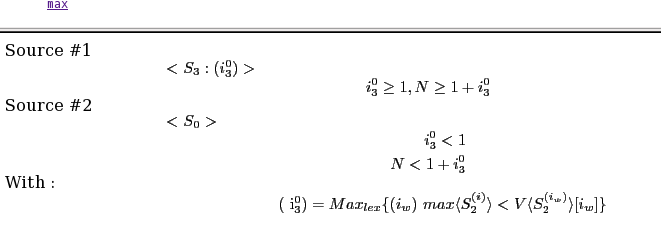
\includegraphics[scale=0.60]{html_tex.png}
\end{center}
\caption{HTML Output for the example of Figure~\ref{pgm:max_vect}}
\label{output:html}
\end{figure}

Here the source of a variable is given in a flat way: the source operation followed by the condition of its validity. The condition is normalised in a DNF form, disjunction (lines) of conjunctions (conjunction of inequations are in a single line).

For example, value of \verb|max| read by $S_4$ during iteration \verb|i| comes from $S_0$ if  $i_3^0 < 1 \vee N < 1 + i_3^0$. This condition ensures that the source is $S_0$ only if no instance of $S_3$ were executed.

For that example, \verb|FADAtool| was not able to compute the exact source operation. But it gives its exact description : $i_3^0 = max_{lex} \{ ( i_w ) / max \langle S_{2}^{(i)} \rangle  < V \langle S_{2}^{(i_w)} \rangle  [ i_w] \}$.

In fact, $i_3^0$ describes the lexicographic maximum (the last write operation) on a set defined by non affine constraints. Here, $i_w$ is an abstract variable used to define the elements of that set.

The source is the {it last} instance of $S_3$ (the lexicographic maximum of the described set) writing in the variable \verb|max|. Since, this set is described by non affine constraints the source can not be evaluated.
It seems pretty printed, but is indeed more complex to read than what we presented so far.
In fact, all non affine entities (variables and array cells) are tagged by the instance of the operation in which they are referenced.
They look like \verb|V <Operation> [Index]| where:
\begin{itemize}
 \item \verb|<Operation>| the operation that references the concerned entity. It looks like: $S_{ID}^{Instance}$  where $ID$ is the identifier of the statement, and $Instance$ its instance.
\item \verb|[Index]| is the array access index. Non-affine laterals with in the index will be tagged in the same way, in that case tagged expressions may not be readable. \verb|A[B[i]+1]| will be tagged as : \verb|A<operation>[B<operation>[i]+1]|.
\end{itemize}


So $max \langle S_{2}^{(i)}\rangle$ should be read: \verb|max| referenced by the instance $i$ of $S_2$. In the same way $V \langle S_{2}^{(i_w)} \rangle  [ i_w]$ is $V[i_w]$ referenced by the instance $i_w$ of $S_2$ (the if-condition).



%\subsubsection{The Instance Wise Dataflow Graph}
\subsubsection{Output: The Instance Wise Dataflow Graph}
Sources of all read variables can be summarised in an instance wise dataflow graph. The dataflow graph produced by \verb|FADAtool| is generated in a \verb|.dot| format (or a \verb|.vcg| format according to the constant \verb|graph_format| in \verb|constants.h|), then automatically converted (if GraphViz installed) into an image. Currently, there is no other output format, we shall appreciate reporting any special format you want the dependence graph will be represented in. 

Here a part of the dataflow graph for the matrix multiply example (Figure~\ref{pgm:matmul}).
\begin{verbatim}
 $ fadatool -i MatMul.c -gc
\end{verbatim}

\begin{center}
 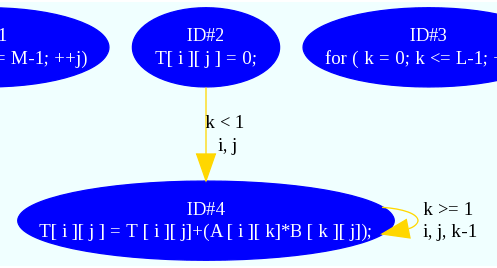
\includegraphics[scale=0.6]{MatMul_DFG.png}
 \end{center}
% \caption{An instance wise dependence graph for program in fig. \ref{pgm:matmul}}
% \label{fig:unfilled_dg}
% \end{figure}

On edges:
\begin{itemize}
 \item The first line gives the condition on validity of the dependence.
 \item The second line gives the function which define the source instance.
\end{itemize}

Here we assume that the read operations are executed during the current iteration vector. Dependent statement instances are identified by an affine function on the read iteration.\\
Let us observe the dependent operations with the operation \verb|ID#4| executed during the iteration \verb|(i, j, k)| (set as the current iteration). One of these dependent operations is \verb|ID#2| executed during the iteration \verb|(i, j)|, the other is another instance of \verb|ID#4| executed during \verb|(i, j, k-1)|.




\section{Using the FADAlib}
We remind that \verb|FADAcore| does not need the AST to perform analysis. Even if we get a C-program as an input, \verb|FADAtool| computes the guarded references (and many other useful information) in order to be able to perform the dependence analysis.

The \verb|FADAtool| (as well as the \verb|FADAlib|) processing is performed in three steps:
\begin{enumerate}
 \item Parse a function and build its AST (Abstract Syntax Tree).
 \item Lower the AST into a vector of ordered and governed references.
 \item Perform the FADA analysis and compute the source of each read memory cell (\verb|FADAcore| step).
\end{enumerate}



% \textbf{What is a lowered governed references ?} We explain that through an example (fig.\ref{pgm:governed})
% \begin{itemize}
%  \item \textbf{Enclosing loops:} the vector of loops enclosing references.
%  \item \textbf{Domain constraints:} are the gard for references. i.e.condition for which references can occur.
%  \item \textbf{Read/Written references:} the list of read and written variables.
% \end{itemize}
% 
% 
% % à mettre un example sur le preprocessing step
% Fig\ref{pgm:governed}. shows a simple example, and how we can extract utile information from the AST of a program (fig.\ref{pgm:governed}). In the real implementation, thing are mush complicated because even controls (here for loops) can reference some memory cells. And that requires creating references for both: controls and assignments.


That gives users three input choices for the \verb|FADAlib| :
\begin{enumerate}
 \item Input C programs (as for \verb|FADAtool|),
 \item Build by C++constructor an AST, and use the lowering functions in order to build references,
 \item or build manually the governed references (a direct input format to  \verb|FADAcore|).
\end{enumerate}


We start by explaining how to build AST and how to lower it into guarded references because it is easier to understand. After that, we demonstrate how to build directly governed references and what changes must be performed, what details have to be respected.

\subsection{First Level of Using FADAlib: Parsing C-like Programs}

\begin{footnotesize}
\begin{lstlisting}[frame=single,framerule=0pt]
#include "fadalib.h"
using namespace fada;

int	main(int argc, char* argv[]){

Program pgm;

try{
	pgm.Parse("your_file_name");
	pgm.ComputeSourcesForAllReadVariables();
	pgm.PrintNormalized(1);
	}
catch(...){
	exit(EXIT_FAILURE);
	}
}
\end{lstlisting}

\end{footnotesize}

Here, we start by parsing a program, then apply the FADA analysis to compute the sources of all read variables, finally print them. The user can set processing and/or printing options accessible by : \verb|Options* Program::GetOptions()|. For example if we want to activate/deactivate the structural analysis, we can do something like:
\begin{verbatim}
 pgm.GetOptions()->processing.apply_structural_analysis=true;
\end{verbatim}


\subsection{Second Level of Using FADAlib: Building an AST by C++ Constructors}
A program is a list of \verb|Statement| objects, which represent statements. A statement can be an \verb|Assignment|, or \verb|Control| (an assignment and control structure respectively). We can build valid statements by using the following C++ methods:

\begin{lstlisting}[frame=single,framerule=0pt]
Statement::Statement(Assignment* __assign) 
\end{lstlisting}
Creates an assignment statement .\\

\begin{lstlisting}[frame=single,framerule=0pt]
Statement::Statement(Control* __control)
\end{lstlisting}
Creates a control statement.\\

\begin{lstlisting}[frame=single,framerule=0pt]
Statement::Enclose(Statement* __s,bool __else_part=false)
\end{lstlisting}
This methods pushes back the statement \verb|__s| in the vector of enclosed statements. If \verb|__else_part| enabled, the method adds \verb|__s| in the else part. \\


\paragraph{Example:} during this section we process the example of Figure~\ref{pgm:max2}:

\begin{figure}

\begin{lstlisting}[frame=single,framerule=0pt]
for(i=0;i<=N;i++) {
   max=0;
   while(max < fct(i))
     if( max > T[i])
        max=T[i];
     else
        max=max;
   }
\end{lstlisting}
\caption{A Simple Input Program Used to Demonstrate How to Build Input Objects for FADAlib}
\label{pgm:max2}
\end{figure}


\subsubsection{Building Assignments}
Assignments are characterised by their left-hand-side (LHS) variable or array cell, and the expression in the right-hand-side(RHS). A valid \verb|Assignment| object can be built using :
\begin{lstlisting}[frame=single,framerule=0pt]
Assignment::Assignment(string array_name,
                  FADA_Index* lhs_index, Expression* rhs) 
\end{lstlisting}
This constructor creates the assignment: \verb|array_name[lhs_index]=rhs|.
\begin{lstlisting}[frame=single,framerule=0pt]
Assignment::Assignment(string var_name, Expression* __rhs) 
\end{lstlisting}
It creates the assignment: \verb|var_name=rhs|.
\begin{lstlisting}[frame=single,framerule=0pt]
Assignment::Assignment(Expression* __rhs) 
\end{lstlisting}
Assignment on no variable, it handles the case of expressions producing no result.

\paragraph{Example}

Below we show how to build the three assignments:

\begin{lstlisting}[frame=single,framerule=0pt]

           // Building assignment "max=0;"
 Assignment* max_equal_zero=new Assignment("max", new Expression (0));

           // Building " max=max;"
 Assignment* max_equal_max=new Assignment("max",new Expression("max"));

           // Building "max=T[i]';"
 Expression* T_i=new Expression("T");
 T_i->AddIndex(new Expression("i"));
 Assignment* max_equal_T_i=new Assignment("max",T_i);

	   //Printing built objects
 max_equal_T_i->Print();cout<<"\n";
 max_equal_max->Print();cout<<"\n";
 max_equal_zero->Print();cout<<"\n";

\end{lstlisting}

\subsubsection{Building Control Structures}
Simple for-loops, while-loops and conditionals and alternatives can be built as a \verb|Control| object using :

\begin{lstlisting}[frame=single,framerule=0pt]
Control::Control(string __lc, Expression* __lb, Expression* __ub)
\end{lstlisting}
builds a for-construct, \verb|__lc| is the loop-counter name where \verb|__lb| and \verb|__ub| are the lower and upper bounds.\\
\begin{lstlisting}[frame=single,framerule=0pt]
Control:: Control(string __lc, Condition* __c)
\end{lstlisting}
builds a while-construct, \verb|__lc| is the loop-counter-name, \verb|__c| is the while-condition.\\

\begin{lstlisting}[frame=single,framerule=0pt]
Control:: Control(Condition* __c)
\end{lstlisting}

We note that loops need loop-counters, used as loop-identifiers, so they have to be distinct each to others. If a loop has not a loop-counter (a typical case of a while-loop), a virtual loop-counter is created: its initial value is set to 1 before starting loop-recurrence, incremented by one at the end of each iteration,  no explicit upper-bound.

\paragraph{Examples:}
Building a for-loop
\begin{lstlisting}[frame=single,framerule=0pt]
 Expression zero= 0;
 Expression N   =(std::string)"N";
 Control* __for=new Control("i",&zero,&N);
 cout<<"\n"<<__for->PrettyPrint_str();

\end{lstlisting}
building a while-loop
\begin{lstlisting}[frame=single,framerule=0pt]
 Expression max=(std::string)"max";
 Expression i=(std::string)"i";

 Expression fct_i=(std::string)"fct";
 fct_i.AddArgument(&i);

 Inequation while_ineq=i < fct_i;
 string virtual_counter="W";
 Control* __while=new Control(virtual_counter,new Condition(&while_ineq));
 cout<<"\n"<<__while->PrettyPrint_str();
\end{lstlisting}
Building an alternative
\begin{lstlisting}[frame=single,framerule=0pt]
 Condition* if_cond=new Condition(new Inequation(&max,FADA_GREATER,T_i));
 Control* __if=new Control(if_cond);
 cout<<"\n"<<__if->PrettyPrint_str();
\end{lstlisting}
\paragraph{Remark:} The variables used in a scope (for example \verb|T_i| in the listing above) are defined and initialised in previous listings. All objects created and initialised are used later.


\subsubsection{Building An AST}
An AST is a special \verb|Statement|. Below we show how to build the AST of the example of Figure~\ref{pgm:max2}:
\begin{lstlisting}[frame=single,framerule=0pt]

 Statement* if_construct= new Statement(__if);
 if_construct->Enclose(max_equal_T_i);
 if_construct->Enclose(max_equal_max,true);

 Statement* while_construct=new Statement(__while);
 while_construct->Enclose(if_construct);

 Statement* for_construct=new Statement(__for);
 for_construct->Enclose(max_equal_zero);
 for_construct->Enclose(while_construct);

 Statement* AST=new Statement();
 AST->Enclose(for_construct);

 cout<<AST->Regenerate_C_Code("\n");

\end{lstlisting}

\subsubsection{Building a Program}

When all statements are created, you have to create a valid \verb|Program| object in order to continue FADA process. A \verb|Program| object has the following properties:
\begin{itemize}
 \item \verb|Program::label| is the name of the program. It will be used as default prefix for output file-names.
 \item \verb|Statement* Program::syntax_tree| is the AST of the program.
\end{itemize}

\paragraph{Example} :

\begin{lstlisting}[frame=single,framerule=0pt]
Program* program=new Program();
program->SetLabel("MyProgramName");
program->SetSyntaxTree(AST);

cout<<"\n"<<program->Generate_C_str();
\end{lstlisting}

\subsubsection{The FADA Processing}
You should know that a pre-process step is performed implicitly when calling the \verb|FADAcore|.
\paragraph{Pre-processing}
The pre-processing performs multiple tasks:
\begin{itemize}
 \item Connecting all AST-objects to each other.
 \item Compute the sequential order between statements.
 \item Be sure that different loop-counter-names are used for different loops, and rename them if necessary.
 \item Identify symbolic constants (scalars which are never modified in the program).
 \item Compute the read and write references and their domains (information required by \verb|FADAcore|), and connect them to the AST (mainly for readability reasons).
 \item Remove symbolic constants and loop counters from the references (useless \verb|FADAcore| computation because their sources are obviously known).
 \item Tag non affine array indexes.
 \item Normalise domain constraints into a disjunction of conjunctions form.
 \item For all references, generate the list of all possible sources, and order them: from the closest (last write operation) to the farthest (first write operation).

\end{itemize}

The pre-processing step fills the following properties which are required for the \verb|FADAcore| processing:
\begin{itemize}
 \item \lstinline|vector<string> Program::global_parameters| : symbolic constants.
 \item \lstinline|vector<References*> Program::normalized_domain| : predicated read and write references.
 \item \lstinline|vector<vector<bool> > Program::sequential_precedence| : the sequential order between statements.
 \item \lstinline|LDemonstrator* Program::global_properties| : properties on irregular while loops.
 \item \lstinline|Read_Reference::schedule| : ordered dependent operations.
\end{itemize}

\verb|vector| here is the regular STL container. All previous properties are private, you have to use appropriate getters to access them.


\paragraph{FADAcore Processing}
The FADA analysis is performed by calling :
\begin{lstlisting}[frame=single,framerule=0pt]
void Program::ComputeSourceForAllReadVariables(void)
\end{lstlisting}
Before performing the analysis, you can specify the processing options using:

\begin{lstlisting}[frame=single,framerule=0pt]
void Program::SetOptions(Options* __otptions);
\end{lstlisting}

For example, if we want to activate the structural analysis :

\begin{lstlisting}[frame=single,framerule=0pt]
Options options;
options.processing.apply_structural_analysis=true;
program->SetOptions(&options);
\end{lstlisting}

\paragraph{Printing Results}
FADA results can be printed using the following methods:
\begin{itemize}
 \item \lstinline|Program::Generate_c(string file_name) | generates a C program for the build AST, result is written in the file \verb|file_name|. Another variant is used to get it in a string (\lstinline|string Program::Generate_C_str()|).
\item \lstinline|Program::PrintNormalized(int __level) | dumps the vector of normalised references. Two levels are usable: 0 to print references with their domain constrains and enclosing loops (available after the preprocessing step), and 1 adds the source of each read variable (available after the FADA processing).\\
\item \lstinline|Program::Generate_GraphViz_Graph(string file_name,...)|  provides a graphviz dot file and transforms it to a png picture if dot is installed.

\item \verb|string Program::ToHtml()|  provides results in HTML pages generated in the directory \verb|Program::options.io.output_directory| after calling this method. And it returns the full file name of the index page.\\
\end{itemize}

% string ToHtml(string dir,bool dot,bool tex,bool flat,bool alphas,bool fuzzy,bool ppts);


Definitions (FADA processing results) are summarised for each statement in \lstinline|References* Statement::references|, directly accessible by calling its getter \lstinline|Statement::GetReferences()|.

A \lstinline|References| object is constituted of :
\begin{itemize}
\item \lstinline|int References::id| : an identifier.
\item \lstinline|vector<Written_Reference*> References::written_variables| : all written variables by this statement.
\item \lstinline|vector<Read_Reference*> References::read_variables| : all read variables.
\item \lstinline|vector<string> References::enclosing_counters| : enclosing loops.
\item \lstinline|Condition* References::domain| : domain constrains.
\item \lstinline|Statement* References::origin| : the original statement (within the built AST).
\end{itemize}

All the above fields are private, you have to use getters to access them, or appropriate constructors to set them.

All these properties are built by the pre-processing mechanism, otherwise, you have to fill them yourself with a correct information.

After a FADA processing the definition of a read memory cell can be accessible by calling the getter \lstinline|Quast* Read_Reference::GetDefinition()|.


\subsection{Third Level of Using FADAlib: Building References and Domain Constraints as a Direct Input to FADAcore}

So far, we presented two ways to prepare an input to perform the FADA analysis on (parsing the source C code, or building an AST). Things were a bit natural an obvious. This section presents the core and the lowest level of the FADA analysis, that is providing direct information to the \verb|FADAcore| layer: this last level is complex and reserved for expert users. We recommend a  previous study of FADA before reading this section. Otherwise, the two previous input levels are sufficient to use the FADA toolkit.

In this third level, we have to set a valid input for the \verb|FADAcore|, that is to build references with  their domains. This requires lot of information to be provided correctly.

For the remaining of the section forget about AST, statements, assignments and control structures. All we want is a list of ordered and guarded references, described by the class \verb|References|.


\subsubsection{Building Valid References Instances}

The information to provide are:
\begin{itemize}
 \item Choose different identifiers for different objects.
 \item Build valid objects for read and written memory cells (\verb|Read_Reference| and \verb|Written_Reference| classes).
 \item Put enclosing loop identifiers in a correct order.
 \item Build the domain constraints:
\end{itemize}

We can set them using the following methods:

\begin{lstlisting}[frame=single,framerule=0pt]
     References::References (int __id,Condition* __domain);
void AddReadReference       (Read_Reference*);
void AddWrittenReference    (Written_Reference*);
void AddInnerCounter        (std::string);
\end{lstlisting}


\paragraph{Example}

Let us reconsider the example of Figure~\ref{pgm:max2}). We can remark:

\begin{itemize}
\item The \verb|for|-construct  does not reference any conflictual variable.
\item \verb|T[i]| is not written in this scope, it is useless to perform the analysis for it.
\item \verb|max| is read by the while-condition, the if-conditions and the third assignment. These three references have exactly the same source.
\end{itemize}


\begin{figure}[!h]
 \begin{verbatim}
      for(i=0;i<=N;i++) {
ID#0:    max=...;
         while(...)
            if(...)
ID#1:         max=...;
            else
ID#2:         max= ... max ...;
   }
 \end{verbatim}
\caption{Simplified Program Example Extracted from Figure~\ref{pgm:max2}}
\label{pgm:simplified_max}
\end{figure}

The FADA processing can be simplified (Figure~\ref{pgm:simplified_max}) by focusing only on the conflictual variables and dropping all uninteresting references. We ignore \verb|T[i]| because it is not written in the program. And we compute only the source of \verb|max| read by the third assignment.
Here how to build \verb|References| objects (We assume some expressions built previously :\verb|max|, \verb|fct_i|,\verb|T_i|):


\begin{lstlisting}[frame=single,framerule=0pt]
Expression i("i");
Expression N("N");
Condition i_ge_0= (Inequation*)&(i>=0);
Condition i_le_N=(Inequation*)&(i <=N);
Condition for_domain= (i_ge_0 && i_le_N);

for_domain.Print();

References* from_assign_1=new References(0,&for_domain);
from_assign_1->AddInnerCounter("i");
from_assign_1->AddWrittenReference(new Written_Reference("max"));


\end{lstlisting}
The first assignment writes one variable \verb|max|, and does not read memory references. It is enclosed by the \verb|i|-loop.
As you can remark, there is no statements, no controls and no AST. All the needed information here  are domains, loops identifiers and references.
\begin{lstlisting}[frame=single,framerule=0pt]

        // Building references for "max=T[i]"
Condition max_less_fct_i= (Inequation*)&(max < fct_i);
Condition max_greater_T_i=(Inequation*)&(max > T_i);

vector<Expression*> instance;
instance.push_back(&i);
instance.push_back(&W);

max_less_fct_i.Instanciate(10,&instance);
max_greater_T_i.Instanciate(20,&instance);
Condition for_while_domain= (for_domain &&  max_less_fct_i );
Condition for_while_then_domain= (for_while_domain && max_greater_T_i);

References* from_assign_2=new References(1,&for_while_then_domain);
from_assign_2->AddWrittenReference(new Written_Reference("max"));
from_assign_2->AddInnerCounter("i");
from_assign_2->AddInnerCounter("W");

\end{lstlisting}
The second assignment writes \verb|max| and reads the reference \verb|T[i]| which is avoided here (never written). These references are enclosed by the \verb|i|-\verb|W|-loop.

\begin{figure}[!h]
\begin{lstlisting}[frame=single,framerule=0pt]

// Building references for "max=max"
Condition for_while_else_domain=
	(for_while_domain && max_greater_T_i.Negate(true));
References* from_assign_3=new References(2,&for_while_else_domain);
from_assign_3->AddWrittenReference(new Written_Reference("max"));
from_assign_3->AddInnerCounter("i");
from_assign_3->AddInnerCounter("W");

Read_Reference* rr=new Read_Reference("max");
/* HERE WE HAVE TO BUILD SOMME EXTRA STUFF*/
from_assign_3->AddReadReference(rr);
\end{lstlisting}
\caption{Building References for the Third Assignment. To be completed in Figure~\ref{code:schedules}}
\label{code:to_be_completed}
\end{figure}
The object \verb|rr| needs advanced stuff, it will be updated in the next section. If we want to print built objects we can execute this code :

\begin{lstlisting}[frame=single,framerule=0pt]
from_assign_1->Print(0);
from_assign_2->Print(0);
from_assign_3->Print(0);
\end{lstlisting}


In the previous listings, we 
\begin{itemize}
\item defined an additional loop counter \verb|W| for the while loop.
\item ignored references coming from the while and if conditions.
\item tagged non affine inequations by empirical IDs. Here we choose \verb|10| for the while condition, and \verb|20| for the if-condition. In fact, IDs are not important them selves, the important is to use the same ID for constraints having the same origin. The \verb|Inequation::Negate(bool)| method, computes a negation of an Inequation, and clones the original right and left hand sides (so result will have the same TAG as the caller, that is very important).
\item creating a \verb|Read_Reference| object needs special stuff, it will be within the next section (Figure~\ref{code:schedules})
\end{itemize}


% Tagging is a way to say that, an inequation, a condition an index or an expression comes from the statement \verb|__stmt| executed during the iteration \verb|__iter|. It is crucial to distinguish between entities having the same name and syntax but express different things.
% 
% If we focus on the case where we check the dependence between $S1$ and $S2$. Some constraints generated by FADA modelling are : $x > 100$, $x <= 100$ which express the validity of $S1$ and $S2$ respectively. They apparently are the negation one to other, but $x$ have not the same value in these two constraints. To distinguish between the two values we will instanciate them to :
% \begin{itemize}
%  \item \verb|x<1,i_w>    >  100|    : to be read like  $x$ read by the first if executed during iteration \verb|i=i_w| is greater than $100$.
%  \item \verb|x<2,i_r>     <= 100|  : should be understood like, $x$ read by the second if during iteration \verb|i=i_r|.
% is less or equal to $100$.
% \end{itemize}
% 
% Here we materialize the difference between different values of the variable $x$.
% 
\subsubsection{Building Read\_Reference Objects}
\paragraph{Read\_Reference}
objects require 
\begin{itemize}
 \item to specify the name of the read variable
 \item a copy of global symbolic constants in (\verb|Read_Reference::global_parameters|)
 \item an appropriate order of all possible source operations \\(\verb|vector<ElementaryDependence*> Read_Reference::schedule|). The idea is to give to the closest operation, the highest priority. And the aim is to stop computing the source when we know for sure that the closest source has been reached
\end{itemize}

You can use these methods to construct Read\_Reference instances :
\begin{footnotesize}\begin{lstlisting}[frame=single,framerule=0pt]
Read_Reference(string);
Read_Reference(string, FADA_Index*);
void SetSchedule(vector<ElementaryDependence*>*);
\end{lstlisting}
\end{footnotesize}
\paragraph{ElementaryDependence}
This class describe a pair of producer/consumer operations. It is used (within \verb|Read_Reference| objects) to order consumers from the closest to the farthest.
Basic \verb|ElementaryDependence| object must have:
\begin{itemize}
 \item A valid couple of read and write operation identifiers.
 \item The deep of precedence (the common iteration). Must be between 0 and the number of common loops.
\end{itemize}


% FADA modeling constraints will be built according to these three integers by : 
% \begin{itemize}
%  \item Recovering constraints to be sure of read and write statements validity.
%  \item Indexes equality, to be sure that read and write operations concerns the same array-cell.
%  \item Lexicographic precedence constraints.
% \end{itemize}

%TODO Marouane, pourquoi tu ne mets pas ces instructions avant ? Pourquoi commences tu par faire un exemple que tu compl�tes apr�s ? 
In order to complete the example of Figure~\ref{code:to_be_completed}, we add the following instructions before building \verb|from_assign_3|:
\begin{figure}[!h]
\begin{footnotesize}\begin{lstlisting}[frame=single,framerule=0pt]
 vector<ElementaryDependence*> closest_sources;
 closest_sources.push_back(new ElementaryDependence(2,2,1));
 closest_sources.push_back(new ElementaryDependence(2,1,1));
 closest_sources.push_back(new ElementaryDependence(2,0,1));  // we can stop here
 closest_sources.push_back(new ElementaryDependence(2,2,0));
 closest_sources.push_back(new ElementaryDependence(2,1,0));
 closest_sources.push_back(new ElementaryDependence(2,0,0));  // no more sources

 rr->SetSchedule(&closest_sources);

\end{lstlisting}
\end{footnotesize}
\caption{Missing Instructions in the Code of Figure~\ref{code:to_be_completed}}
\label{code:schedules}
\end{figure}

\subsubsection{FADAcore Processing}
After building all references, you can prepare the FADAcore processing in a pre-processing step.

\paragraph{Pre-processing}
Before applying the FADAcore analysis, we have to :
\begin{itemize}
 \item Instantiate read, and write array indexes.
 \item Normalise domain constraints and sort them into affine and non affine constraints.
 \item Compute symbolic constants.
 \item Compute some loop properties.
 \item Indicate the textual order between statements.
\end{itemize}

The first three tasks can be performed by the global function :
\begin{footnotesize}\begin{lstlisting}[frame=single,framerule=0pt]
Preprocess (vector<References*>* __ref, vector<string>* __constants);
\end{lstlisting}
\end{footnotesize}

The two last tasks are in charge of the user, explained below.

\subparagraph{Compute Loop Properties}
Loop properties are summarised within a \verb|LDemonstrator| object. Regular instructions are :
\begin{footnotesize}\begin{lstlisting}[frame=single,framerule=0pt]
LogicalClause*	LoopProperty(vector<string>* counters, string c, Inequation* loop_const);
\end{lstlisting}
\end{footnotesize}
The first method generate the following clause : \\
\begin{math}
 \forall counters, c1, c2, loop\_const(counters,c1), c2 \leq c1 \Rightarrow loop\_const(counters, c2)
\end{math}
where :
\begin{itemize}
 \item counters : the vector of loops enclosing the concerned loop.
 \item c : the loop counter of the concerned loop.
 \item loop\_const : the non affine inequation coding the domain of the loop.
\end{itemize}

The clause describes the fact that if the loop condition is upheld for an iteration, so it is so for all previous iterations.

For the example of Figure~\ref{pgm:simplified_max}, the \verb|FADAlib| instructions used to build properties on the while loops are:

\begin{footnotesize}\begin{lstlisting}[frame=single,framerule=0pt]
LDemonstrator* ppts=new LDemonstrator();
vector<string> enclosing_loops;
enclosing_loops.push_back("i");
ppts->PUSHBACK(IrregularLoop(&enclosing_loops,"W", &max_less_fct_i));
\end{lstlisting}
\end{footnotesize}
\subparagraph{Sequential Textual Order between Statements}
The textual sequential order between references must be indicated correctly, because this information is critical for processing step. The matrix of sequential order of our simplified references of Figure~\ref{pgm:simplified_max} is: 

\begin{footnotesize}\begin{lstlisting}[frame=single,framerule=0pt]
vector<vector<bool> > sequential_order;
sequential_order.resize(3);
sequential_order[0].resize(3); sequential_order[1].resize(3); sequential_order[2].resize(3);
sequential_order[0][0]=false;
sequential_order[0][1]=true;
sequential_order[0][2]=true;
sequential_order[1][0]=false;
sequential_order[1][1]=false;
sequential_order[1][2]=false;
sequential_order[2][0]=false;
sequential_order[2][1]=false;
sequential_order[2][2]=false;
\end{lstlisting}\end{footnotesize}

That means in the simplified program in Figure~\ref{pgm:simplified_max}:
\begin{itemize}
 \item References \verb|ID#0| precede those from \verb|ID#1| and \verb|ID#2|
 \item There is no sequential order between \verb|ID#1| and \verb|ID#2|, because they come from different branches of an \verb|if-then-else| construct.
\end{itemize}

After doing a correct pre-processing step, FADAcore can be called as explained in the next paragraph.
\paragraph{FADAcore Processing}
By simply calling:
\begin{footnotesize}
\begin{lstlisting}[frame=single,framerule=0pt]
void References::ComputeDefinitions(vector<string>* constants,
                     vector<References*>* all_references,
                     vector<vector<bool> >* sequential_order,
                     LDemonstrator* loops_ppts,
                     Options* options);
\end{lstlisting}
\end{footnotesize}

\subparagraph{Example} to finalise the processing, we add these instructions 
\begin{footnotesize}
\begin{lstlisting}[frame=single,framerule=0pt]
Options options;
vector<string>* constants=new vector<string>();
constants->push_back("N");
vector<References*> * all_ref=new vector<References*>();
all_ref->push_back(from_assign_1);
all_ref->push_back(from_assign_2);
all_ref->push_back(from_assign_3);
for(vector<References*>::iterator it=all_ref->begin(); it != all_ref->end(); ++it)
   (*it)->ComputeDefinitions(constants, all_ref,&sequential_order,ppts,&options);
\end{lstlisting}
\end{footnotesize}

\paragraph{Printing Results}
A simple pretty print loop looks like:
\begin{footnotesize}
\begin{lstlisting}[frame=single,framerule=0pt]
for(vector<References*>::iterator it=all_ref->begin(); it != all_ref->end(); ++it)
   (*it)->Print(1);
\end{lstlisting}
\end{footnotesize}
% After building affine constraints, the exact source (maximum lexicographic) is computed in \verb|Quast* ElementaryDependence::quast|. Otherelse, an extra stuff is done :
% 
% \begin{itemize}
%  \item Relax the non affine constrains, and check whether affine ones are upheld.
%  \item If it is the case, a parameter of the maximum is computed in 
% \begin{lstlisting}[frame=single,framerule=0pt]
% vector<string> ElementaryDependence::parameter_of_maximum
% \end{lstlisting}
% and some properties on it are given in
% \begin{lstlisting}[frame=single,framerule=0pt]
% SimpleDemonstrator* ElementaryDependence::properties 
% \end{lstlisting}
% 
% These properties will be used later in order to perform the FADA advanced analysis.
% \end{itemize}
% 
% All that is done by the simple call of 
% 
% \begin{lstlisting}[frame=single,framerule=0pt]
% void 
% ElementaryDependence::BuildAndComputeMax(vector<string>*__read_iteration, 
%                vector<string>* __global_parameters, Program* __pgm)
% \end{lstlisting}
% 
% where :
% \begin{itemize}
%  \item \verb|__read_iteration| is a fixed iteration obtained by adding the suffix \verb|current_| to the enclosing counters (we strongly recommend the function \\ \verb|vector<string>  ParameterizeReadIteration(vector<string>* __lc)| in \verb|global.cpp|).
%  \item \verb|__global_parameters| : are the read-only scalars of the entire program.
%  \item \verb|__pgm| is used for one only aim : check wether there is a textual order between two statements, for that the current implementation need the AST to check out that. See : 
% \begin{lstlisting}[frame=single,framerule=0pt]
% bool Program::IsTextuallyBefore(int __id1, int __id2,
%                                  vector<string>* common_loops)|). 
% \end{lstlisting}
% 
% \end{itemize}
% 
% 
% 
% Here we can say that both $S1$ and $S2$ have a textual order with S3, so we have to consider the deep 1 if $S1$ and\/or $S2$ are possible sources for a variable read by $S3$. However, there is no textual order between $S1$ and $S2$, it is meaningless to check whether there is a dependence between then for the same iteration.
% Relieving this kind of information can implicate a faster FADA analysis, and eventually much more precise results.
% 
% 
% After building a correct schedule in the right order for all read variables in the entire program, we can proceed to the evaluation of their sources by calling \verb|void Program::ComputeSourcesForAllReadVariables(bool)|, results are provided in \verb|Read_Reference::definition|.
% 




\section{Conclusion}
{\it FADA Toolkit} is a partial implementation of the FADA code analysis \cite{barthou_thesis}. \verb|FADAlib| is a C++ library, with a C++ API. The user may use it as an external library for data dependence analysis. The input of \verb|FADAlib| is either an AST (built with C++ classes) or low level information of references and domains (also built with C++ classes). 

\verb|FADAtool| is a command line invocation of FADA analysis. It parses a C-like program, computes its data dependences and print them to the user on the console and/or in HTML pages.

Currently, both  \verb|FADAlib| and  \verb|FADAtool| are open source software intended for academic research purposes. In some cases, the computation time of these tools is expensive because of the complexity of data flow analysis of irregular programs, and also because of the internal usage of PIP solver. The quality of FADAlib would be improved step by step in the future. 

One of our future plans is to connect FADAlib to gcc, especially to a branch called Graphite. 

\section*{License}
This program is free software: you can redistribute it and/or modify
it under the terms of the LGPL GNU General Public License as published by
the Free Software Foundation, either version 3 of the License, or(at your option) any later version.

This program is distributed in the hope that it will be useful,
but WITHOUT ANY WARRANTY; without even the implied warranty of
MERCHANTABILITY or FITNESS FOR A PARTICULAR PURPOSE.  See the
GNU General Public License for more details.

You should have received a copy of the LGNU Libray General Public License
along with this program.  If not, see \texttt{http://www.gnu.org/licenses}

\section*{Contributors}
Please send suggestions, bug reports and remarks to:
\begin{enumerate}
 \item \texttt{Marouane.Belaoucha@prism.uvsq.fr}, PhD student, principal contributor. 
 \item \texttt{Denis.Barthou@prism.uvsq.fr}, Associate professor, FADA's father. 
 \item \texttt{Sid.Touati@uvsq.fr}, Associate professor, supervisor.

We would like to thank Christophe Alias for his support, as well as for having accepted to share his efforts with us. FADAlib was largely inspired by his work on \textbf{BeeCl@ck}.
\end{enumerate}


\bibliographystyle{plain}

\bibliography{ma_bdd}


\end{document}
